\section*{Inhalte, Ringe und Halbringe}

\begin{karte}{Ring}
	Sei \(X\) eine Menge. Ein System \(\mathcal{R} \subset \mathcal{P}(X) \) heißt \textit{Ring}, falls 
	\begin{enumerate}
		\item \( \emptyset \in \mathcal{R} \).
		\item \( A,B \in \mathcal{R} \Rightarrow A\setminus B \in \mathcal{R} \).
		\item \( A,B \in \mathcal{R} \Rightarrow A \cup B \in \mathcal{R} \).
	\end{enumerate}
	Fordert man zusätzlich noch \(X \in \mathcal{R}\), dann ist \(\mathcal{R}\) eine Algebra.
\end{karte}

\begin{karte}{Stabilität algebraischer Objekte}
	Sei \( \mathcal{A} \subset \mathcal{P}(X) \) ein algebraisches Objekt. 
	Dann ist \( \mathcal{A} \)
	\begin{itemize}
		\item \(\cap\)-stabil, wenn \( A,B\in \mathcal{A} \Rightarrow A \cap B \in \mathcal{A} \).
		\item \(\cup\)-stabil, wenn \( A,B\in \mathcal{A} \Rightarrow A \cup B \in \mathcal{A} \).
		\item \(\setminus\)-stabil, wenn \( A,B\in \mathcal{A} \Rightarrow A \setminus B \in \mathcal{A} \).
		\item \(\sigma\)-\(\cap\)-stabil, wenn \( (A_j)_{j\in\N} \subset \mathcal{A} \Rightarrow \bigcap_{j\in\N} A_j \in \mathcal{A} \).
		\item \(\sigma\)-\(\cup\)-stabil, wenn \( (A_j)_{j\in\N} \subset \mathcal{A} \Rightarrow \bigcup_{j\in\N} A_j \in \mathcal{A} \).
		\item \( (\cdot)^C\)-stabil, wenn \( A \in \mathcal{A} \Rightarrow A^C \in \mathcal{A} \).
	\end{itemize}
\end{karte}

\begin{karte}{Algebraische Objekte}
	\centering
	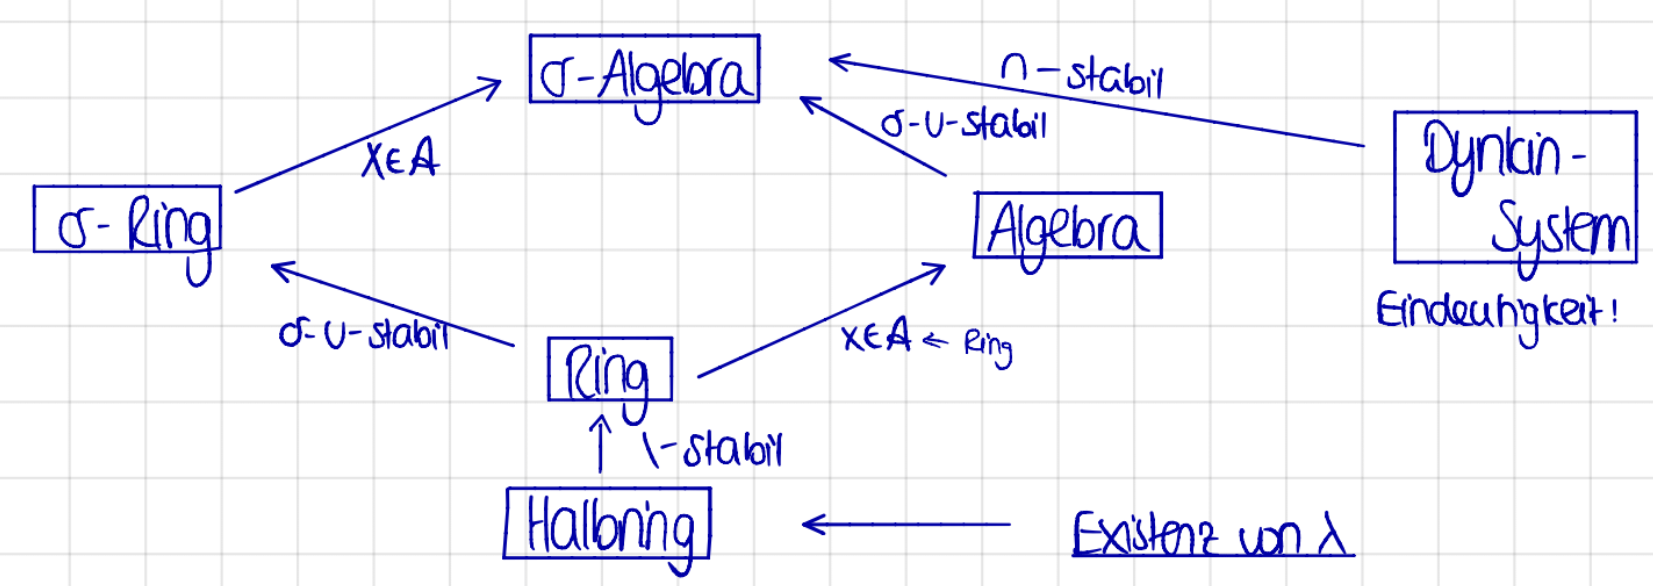
\includegraphics[height=0.33\textwidth]{algebraische-objekte-zusammenhang.png}
\end{karte}

\begin{karte}{Inhalt}
	Sei \( \mathcal{R} \subset \mathcal{P}(X) \) (nicht notwendigerweise ein Ring). Dann heißt 
	\( \abb{\mu}{\mathcal{R}}{[0,\infty]} \) Inhalt, falls 
	\begin{enumerate}
		\item \( \mu(\emptyset) = 0 \).
		\item Für endlich viele disjunkte Mengen \( A_1 ,\ldots, A_n \) gilt 
		\[ \mu \left( \bigcup_{j=1}^n A_j \right) = \sum_{j=1}^n \mu(A_j). \]
	\end{enumerate}
	Jedes Prämaß ist ein Inhalt mit \( A_{n+1}, \ldots = \emptyset \).
\end{karte}

\begin{karte}{Halbring}
	Ein Mengensystem \( \mathcal{H} \subset \mathcal{P}(X) \) ist ein \textit{Halbring}, falls 
	\begin{enumerate}
		\item \( \emptyset \in \mathcal{H} \).
		\item \( A, B \in \mathcal{H} \Rightarrow A \cap B \in \mathcal{H} \).
		\item \( \forall A,B\in \mathcal{H} \) gibt es disjunkte \( C_1,\ldots, C_n \in \mathcal{H} \) 
		mit \( A \setminus B = \bigcup_{j=1}^n C_j \).
	\end{enumerate}
	Ist \( \mathcal{E} \subset \mathcal{P}(X) \), so heißt 
	\[ \mathcal{R}(\mathcal{E}) 
	:= \bigcap_{\substack{\mathcal{R} \subset \mathcal{P}(X) \text{ ist Ring}\\ \mathcal{E} \subset \mathcal{R}}} \mathcal{R} \]
	der von \( \mathcal{E} \) erzeugte Ring.\\
	Für jedes \( d\in \N \) ist \(J^d\), die Menge der halboffenen Intervalle in \(\R^d\), ein Halbring (auch \(J_\Q^d\)). 
\end{karte}

\begin{karte}{Halbringprodukt}
	Sind \( \mathcal{H}_1, \mathcal{H}_2 \) Halbringe in \(X\) und \(Y\), so ist \( \mathcal{H}_1 * \mathcal{H}_2 := \set{ A\times B \;|\; A\in \mathcal{H}_1, B\in \mathcal{H}_2 } \subset \mathcal{P}(X,Y) \) ein Halbring in \(X\times Y\).
\end{karte}

\begin{karte}{Halbring Verschärfung der Definition}
	Sind \( A, B_1, \ldots, B_n \) Elemente in einem Halbring \( \mathcal{H} \), 
	so gibt es disjunkte Mengen \( C_1, \ldots, C_m \in \mathcal{H} \) mit 
	\[ A \setminus \left( \bigcup_{j=1}^n B_j \right) = \bigcup_{j=1}^m C_j. \]
\end{karte}

\begin{karte}{Erzeugung eines Ringes durch Halbring}
	Der von einem Halbring \( \mathcal{H} \) erzeugte Ring \( \mathcal{R}(\mathcal{H}) \) ist gegeben durch 
	\[ \mathcal{R} = \mathcal{R}(\mathcal{H}) := \set{ \bigcup_{j=1}^n \;|\; n\in\N, A_1, \ldots, A_n \in \mathcal{H} \text{ disjunkt} }. \]
\end{karte}

\begin{karte}{Nullmenge}
	Für \(\mu\) ist \( M\in \mathcal{A} \) eine Nullmenge, falls \( \mu(M) = 0 \).
\end{karte}

\begin{karte}{Erster Fortsetzungssatz}
	Sei \( \abb{\mu}{\mathcal{H}}{[0,\infty]} \) ein Inhalt auf einem Halbring \(\mathcal{H}\) 
	und \( \mathcal{R} \) der von \(\mathcal{H}\) erzeugte Ring.\\
	\(\Rightarrow \exists !\) Fortsetzung \( \abb{\nu}{\mathcal{R}}{[0,\infty]} \) von \(\mu\) 
	zu einem Inhalt auf \(\mathcal{R}\) und zwar ist 
	\[ \nu(A) = \sum_{j=1}^n \mu(A_j), \]
	falls \(A \in \mathcal{R}\) die endliche Vereinigung der disjunkten Mengen \(A_1,\ldots,A_n\in\mathcal{H}\) ist.\\
	Ferner gilt: \(\nu\) ist ein Prämaß auf \(\mathcal{R}\) 
	\(\Leftrightarrow\) \(\mu\) ist ein Prämaß auf \(\mathcal{H}\).
\end{karte}

\begin{karte}{Lebesguesches Prämaß}
	Das lebesguesche Prämaß \( \abb{\lambda^d}{J^d}{[0,\infty)} \) auf \(J^d\) 
	mit \(I = \prod_{j=1}^d [a_j,b_j) \in J^d \) ist definiert durch 
	\[ \lambda^d(\emptyset) := 0, \quad \lambda^d(I) := \prod_{j=1}^d (b_j - a_j). \] 
\end{karte}